%%  Assignment 5 for CSC263H1, Fall 2015,
%%  at the University of Toronto.
%%
%%  Copyright (c) 2014 Toniann Pitassi <toni@cs.utoronto.ca>
%%  last updated at 09:02 (EDT) on Mon  9 Mar 2015
%%
%%  CC BY-SA 4.0
%%  This work (the current file named 'A2handout.tex') is licensed under
%%  the Creative Commons Attribution-ShareAlike 4.0 International License.
%%  To view a copy of this license, visit
%%      http://creativecommons.org/licenses/by-sa/4.0/
%%  or send a letter to: Creative Commons, 444 Castro Street, Suite 900,
%%  Mountain View, California, 94041, USA.
%%  This is a human-readable summary of (and not a substitute for) the
%%  license.
%%  You are free to:
%%      Share -- copy and redistribute the material in any medium or format
%%      Adapt -- remix, transform, and build upon the material for any
%%          purpose, even commercially.
%%      The licensor cannot revoke these freedoms as long as you follow the
%%          license terms.
%%  Under the following terms:
%%      Attribution -- You must give appropriate credit, provide a link to
%%          the license, and indicate if changes were made. You may do so in
%%          any reasonable manner, but not in any way that suggests the
%%          licensor endorses you or your use.
%%      ShareAlike -- If you remix, transform, or build upon the material,
%%          you must distribute your contributions under the same license as
%%          the original.
%%      No additional restrictions -- You may not apply legal terms or
%%          technological measures that legally restrict others from doing
%%          anything the license permits.
%%  Notices:
%%      You do not have to comply with the license for elements of the
%%      material in the public domain or where your use is permitted by an
%%      applicable exception or limitation.
%%      No warranties are given. The license may not give you all of the
%%      permissions necessary for your intended use. For example, other
%%      rights such as publicity, privacy, or moral rights may limit how you
%%      use the material.

\RequirePackage[l2tabu,orthodox]{nag}  % warn about common LaTeX pitfalls
\RequirePackage[ascii]{inputenc}  % input is 7-bit ASCII
\RequirePackage{fixltx2e}  % fix LaTeX2e kernel bugs

\documentclass[11pt,twoside]{article}
\usepackage{calc}  % arithmetic in length parameters
\usepackage{color}  
\usepackage{tikz}
\usepackage{enumitem}  % more control over list formatting
\usepackage{fancyhdr}  % simpler headers and footers
\usepackage[margin=1in]{geometry}  % page layout
\usepackage{lastpage}  % for last page number
\usepackage{relsize}  % easier font size changes
\usepackage[normalem]{ulem}  % smarter underlining
\usepackage{url}  % verb-like typesetting of URLs
%\usepackage{xfrac}  % nicer looking simple fractions for text and math
\usepackage{amsmath}
\usepackage{amssymb}

% Set up fonts.
\usepackage[T1]{fontenc}  % use true 8-bit fonts
\usepackage{slantsc}  % allow slanted small-caps
\usepackage{microtype}  % perform various font optimizations
% Version 1.2 (2015/02/08) of newpxtext messes up \textsl so skip it...
% Use Palatino-based monospace instead of kpfonts' default.
%\usepackage{newpxtext}
%\ttfamily
%\DeclareFontShape{T1}{\ttdefault}{m}{scsl}{<->ssub*\ttdefault/m/sc}{}
%\DeclareFontShape{T1}{\ttdefault}{b}{scsl}{<->ssub*\ttdefault/b/sc}{}
% "Kepler" fonts.
\usepackage[nott,notextcomp]{kpfonts}
% Use curvier Latin Modern brackets instead of kpfonts' glyphs.
\DeclareSymbolFont{lmsymb}     {OMS}{lmsy}{m}{n}
\DeclareSymbolFont{lmlargesymb}{OMX}{lmex}{m}{n}
\DeclareMathDelimiter{\rbrace}{\mathclose}{lmsymb}{"67}{lmlargesymb}{"09}
\DeclareMathDelimiter{\lbrace}{\mathopen}{lmsymb}{"66}{lmlargesymb}{"08}

% Page layout: stretch text to fill up page.
\addtolength\footskip{.25\headheight}
\flushbottom

% Common macros.
\input{macros-263}

% Headings.
\pagestyle{fancy}
\let\headrule\empty
\let\footrule\empty
\lhead{CSC\,263\,H1}
\chead{\large\scshape Assignment \#\,5}
\rhead{\scshape Fall 2015}
\lfoot{\scshape Dept.\@ of Computer Science, University of Toronto,
       St.~George Campus}
\cfoot{}
\rfoot{\scshape page \thepage\space of \pageref{LastPage}}


\begin{document}

\noindent
\strong{Worth:}  8\%
\hfill
\strong{Due:}  By 5:59pm on Tuesday 31 November\\[2ex]
\strong
   {Remember to write
    the \emph{full name} and \emph{student number}
    of \emph{every group member}
    prominently on your submission.}

\medskip

\noindent
\rule{\textwidth}{.5pt}\\[1ex]
\begingroup\slshape
    Please read and understand the policy on Collaboration
    given on the Course Information Sheet.
    Then, to protect yourself,
    list on the front of your submission
    \strong{every} source of information
    you used to complete this homework
    (other than your own lecture and tutorial notes).
    For example, indicate clearly
    the \strong{name} of every student from another group
    with whom you had discussions,
    the \strong{title and sections} of every textbook you consulted
    (including the course textbook),
    the \strong{source} of every web document you used
    (including documents from the course webpage),
    \etc.\par
        For each question, please write up detailed answers carefully.
    Make sure that you use notation and terminology correctly, and
    that you explain and justify what you are doing.
    Marks \strong{will} be deducted
    for incorrect or ambiguous use of notation and terminology, and
    for making incorrect, unjustified, ambiguous, or vague claims
    in your solutions.
\endgroup\\
\rule{\textwidth}{.5pt}
% If you use this file as a template for your solution, please remove
% (or comment out) the block above!

\begin{enumerate}[leftmargin=0pt]

\item
Let $x_1,\ldots,x_n$ be $n$ be a list of $n$ people who have applied
for a job at Google. They are interviewed in pairs: if $x_i$ and $x_j$
are interviewed together, one of them is chosen to be more qualified. 
You are given a list of outcomes of $m$ interviews, each of the form
"candidate $x_i$ is more qualified than candidate $x_j$"
Your task is to order the job candidates, with the best candidate first.
Specifically, if $x_i$ is more qualified than $x_j$ (as the result
of the outcome of some interview), then you must place candidate $x_i$
ahead of $x_j$ in the ordering.
%Use what you learned from CSC263 to answer the following questions.
\begin{enumerate}[label=(\alph*)]
        \item How do you model this problem using a graph? Assume that all
                graphs in this problem set are implemented using adjacency list.
        \item How do you determine whether it is possible at all to arrange
                all candidates in a line such that all constraints are satisfied? Explain your
                algorithm in clear English, and analyse its worst-case running time.
        \item Assuming such arrangement is possible, how do you compute an
                actual arrangement? Explain your algorithm in clear English, and
                analyse its worst-case running time.
\end{enumerate}
\textcolor{red}{$answer:$}
\begin{enumerate}
% a
\item We construct  a directed graph  $G(V,E)$ with the following rules,
	\begin{itemize}
	\item Construct a graph with $n$ nodes, that is  $G(V,E)$ where $V =\{ x_1,\ldots,x_n \} \ and \ E = \emptyset$. Each node stands for a  candidate. Using adjacency list it would be create $n$ empty list of size $m$ and list $A[i]$ is for vertex $x_i$.
	\item For each of the $m$ outcomes, we add a edge $\overrightarrow{x_ix_j}$ to $E$, if  outcome says "candidate $x_i$ is more qualified than candidate $x_j$". In other words, stores $x_j$ in $A[i]$.
	\end{itemize}
	We attempt the solve the problem using topological sort such that the vertices are in an order that all edges are pointing to the right side. Then every candidate is more qualified than the candidates on its left.
% b
\item Arranging all candidates in a line such that all constraints are satisfied means such topological sort exist, which means the graph is acyclic. \\
First we construct the graph by the rules mentioned in $(a)$. Then we do a depth first search, check for cycle. If the graph is acyclic then it is possible to arrange all candidates, otherwise not possible. \\ 
The run time for construct the graph $G(V, E)$ would take $\mathcal O (m)$, where $|V| = n$ and $|E| = m$. DFS check for cycle using adjacency list would take $\mathcal O (n+m)$. Hence, the worst case runtime is 
$\mathcal O (n+m)$.
% c
\item 
We can compute an actual arrangement by topological sort such that the vertices are in an order that all edges are pointing to the right side. Since all edges are pointing to the right side which means every candidate is more qualified than the candidates on its left. Then the order generated by the topological sort would be a valid arrangement. \\
First we construct the graph $G(V,E)$ which takes $\mathcal O (m)$, then call DFS(G) to compute finishing times $f[x_i]$ foreach vertex $x_i$. And as each vertex is finished, insert it on to the front of a linked list return the linked list of vertices, this would take  $\mathcal O (n+m)$. Hence, the worst case runtime is $\mathcal O (n+m)$.

\end{enumerate}

%% question 2
\item
Let $G = (V,E)$ be a weighted undirected connected graph that contains a
cycle, and let $e$ be the maximum-weight edge among all edges in the cycle.
\strong{Prove} that there exists a minimum spanning tree of $G$ which does
NOT include $e$. \\
% solution
\\
\textcolor{red}{$Proof:$}
	\begin{itemize}[label = {}]
		\item Suppose $v_1v_2...v_n v_1$ is the circle mentioned in the question, and  $v_i, v_j$	
			are the vertices adjacent to edge $e$, which with maximum-weight among all edges in 
			the cycle. Let $T$ be any minimum weight spanning tree of $G$ .

		\item If T does not contain edge $e$ then we are done.
		\item Now suppose $T$ contain edge $e$, then $T-e$ has two connected component $A, B$, and 
			each of them is a tree. 
		\item Since $v_1v_2...v_n v_1$ form a circle, then there must be some edge $e'$ other than $e$ with 
		two ends point $u,v$ are in $A,B$ separately. Otherwise, $v_1v_2...v_n v_1$ could not form a circle. 
		\item Then connect $A, B$ with edge $e'$, then we get  $T-e+e'$. 
		\item Since $A, B$ are two connected component then $T-e+e'$ is a spanning tree of $G$. Also 
		according to the question we know that weight of $e'$ is no more than $e$; hence, $T-e+e'$  is also a
		minimum-weight spanning tree of $G$.
	\end{itemize}


\item
Consider a list of cities $c_1, c_2, \dots, c_n$.  Assume we have
a relation $R$ such that, for any $i,j$, $R(c_i, c_j)$ is 1 if cities
$c_i$ and $c_j$ are in the same province, and 0 otherwise.

\begin{enumerate}
\item
If $R$ is stored as a table, how much space does it require?


\item
Using a disjoint set ADT, write pseudo-code for an algorithm
that puts each city in a set such that $c_i$ and $c_j$ are in the same
set if and only if they are in the same province.
(That is, you can assume that you have some implementation
of the basic disjont set operations, MAKE-SET, FIND-SET, and UNION.)


\item
When the cities are stored in the disjoint set ADT, if you are
given two cities $c_i$ and $c_j$, how do you check if they are in the
same province?


\item
If we use trees with the rank heuristic, what is the worst-case
running time of the algorithm from (b) (Hint: the unions from your
algorithm probably have a special form).  Explain.


\item
If we use trees without the rank heuristic, what is the worst-case
running time of the algorithm from (b).  Explain.  Are there more
worst-case scenarios than in (d)?

\end{enumerate}
\textcolor{red}{$Answer$}                                                                                                                                                                                                   
%question 3 
\begin{enumerate}

% a 
\item If $R$ is stored as a table, then we have to store the relation between any two cities.
Hence, it requires at least ${n \choose 2} = \frac{n(n-1)}{2}$ brackets.
% b
\item
	\proc{construct:}
	\begin{enumerate}[label = {\arabic*}]
	\item first we do a MAKE-SET for each city, and we get $c_1, c_2, \dots, c_n$, n sets
	\item	for $c_i$ in $c_1, c_2, \dots, c_n$:
	\item \hskip2pc  for $c_j$ in $c_{i+1}, c_{i+2}, \dots, c_n$:
	\item  \hskip4pc  if $R(c_i, c_j)$ and FIND-SET($c_i$)  $\neq$ FIND-SET($c_j$): 
	\item  \hskip6pc  UNION($c_i$, $c_j$)
	\end{enumerate}
	
	The function \proc{construct} loops through every pair of $(c_i,c_j)$.   If $c_i$ and $c_j$ are in the same province but different sets, then UNION($c_i$, $c_j$).  Hence, every two cities which are in the same province are in the same set.
% c
\item Since $R$ is clearly a equivalence relation, then to check if any two given sets $c_i$ and $c_j$ are stored in the same set, we call FIND-SET on $c_i$ and $c_j$. If they return the same representative, then they are in the same set otherwise not.
% d
\item
	$Claim:$ If we use trees with the rank heuristic, then every disjoint set we get from \proc{construct} has height no more than $1$. \\
    	  \begin{center}
                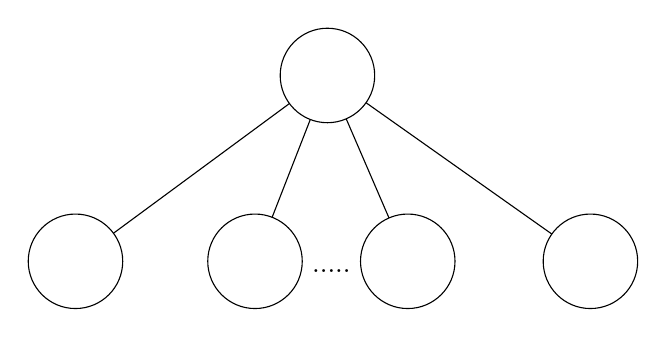
\begin{tikzpicture}[scale=0.2]
                \tikzstyle{every node}+=[inner sep=0pt]
                \draw [black] (34.9,-11.7) circle (3);
                \draw [black] (18.9,-23.5) circle (3);
                \draw [black] (30.3,-23.5) circle (3);
                \draw [black] (40,-23.5) circle (3);
                \draw [black] (51.6,-23.5) circle (3);
                \draw [black] (32.49,-13.48) -- (21.31,-21.72);
                \draw [black] (36.09,-14.45) -- (38.81,-20.75);
                \draw [black] (37.35,-13.43) -- (49.15,-21.77);
                \draw [black] (33.81,-14.5) -- (31.39,-20.7);
                \draw (35.15,-24) node [below] {$.....$};
                \end{tikzpicture}
        \end{center}
        It is sufficient to show after each iteration of the outer for loop every disjoint set has height no more than $1$. We prove this by induction on the number of iterations of the outer for loop. 
	\begin{itemize}[label = {}]
	\item Base Case: $i = 0$, every disjoint set contains just one element; hence, has height $0$. \\
	\item Induction Hypothesis: After  $k$ iteration, every disjoint set has height no more than $1$. \\
	\item Induction Step: At $(k+1)_{th}$ iteration if \proc{construct} calls UNION($c_i$, $c_j$), by induction
	 hypothesis, we know set contains $c_i$  has height no more than $1$.  
	\item Also, because FIND-SET($c_i$) $\neq$ FIND-SET($c_j$) then set $c_j$ must has height $0$. If set $c_j$ does not have height $0$, which means at some previous iteration (i.e $m_{th}$ where $m<i$), $R(c_m, c_j)$, then clearly $R(c_m, c_i)$ as well. It contradicts  with FIND-SET($c_i$) $\neq$ FIND-SET($c_j$), then set $c_j$ must has height $0$; therefore, UNION($c_i$, $c_j$) generates a set of height no more than $1$. Induction follows.
	 \item
	 \end{itemize}
	Now let's discuses the worst case runtime. It is clear that $line \# 1, \#2$ always execute $n$ times. Since  \proc{construct} checks all pair of $(c_i,c_j)$, $line \#3, \#4$ always executes $\frac{n^2-n}{2}$ times. 
	From the claim we know that unions from \proc{construct} all have height no more than $1$; hence, FIND-SET and  UNION take constant time. Then no matter in which cases $line \# 1$ up to $\#4$ always take the same time. \\ 
	The worst case scenario occurs only when $line \#5$ executes the most which is  $c_1, c_2, \dots, c_n$ are all in the same province.   Then $line \#5$ executes $n-1$ times takes $\Theta(n)$. The total runtime is still dominated by $line \#3, \#4$. Hence, the worst case run time is $\Theta (n^2)$ more precisely $ n^2+3n $.
%e
\item	 
If we use trees without the rank heuristic, the UNION takes constant time. Also the runtime for $line \# 1, \#2, \#3$ is fixed for any cases. Hence, the worst-case runtime depends on the total runtime of $line \# 3$,  			
	\begin{center} if $R(c_i, c_j)$ and FIND-SET($c_i$)  $\neq$ FIND-SET($c_j$) \end{center}
which in other words depends on the height of the tree.\\

Hence, worst-case scenario occurs only when all cities are in the same provence that is we will have a tree of height $n-1$.

We know that $line \# 3$ will be executed $\frac{n^2-n}{2}$ times. After the first $n$ times we will have a tree of height $n-1$ then the rest $\frac{n^2-3n}{2}$ times would take $(n-1)\frac{n^2-3n}{2}$. Therefore,
worst-case runtime is $\Theta(n^3)$.\\
Like we already discussed, the worst-case scenario happens for $d$ only when all cities are in the same province. Same for $e$; therefore, The worst-case scenario for both $d$ and $e$ are the same.
\end{enumerate}

\end{enumerate}

\end{document}
